\section{Dise\~no de alto nivel}
\label{hld}
\subsection{Interfaces - Responsabilidades - Colaboradores}
En esta secci\'on se presentan las principales interfaces que intervienen en el
sistema, sus respectivas responsabilidades y colaboradores. En la
Figura~\ref{uml:hld} se puede ver el diagrama de clases correspondiente.
\begin{figure}  
  \centering
  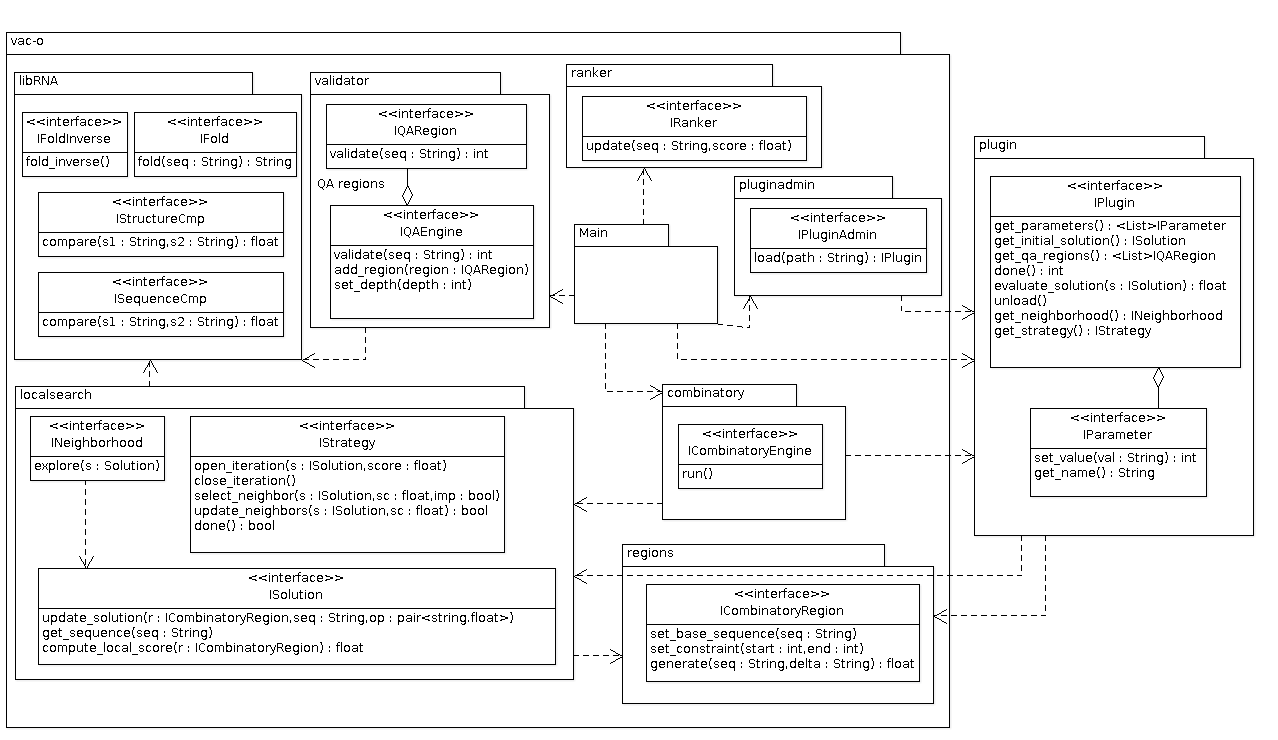
\includegraphics[scale=0.5, angle=90]{hld.png}  
  \caption{UML - Interfaces}
  \label{uml:hld}
\end{figure} 

  \subsubsection{IPluginAdmin}
    \paragraph{Responsabilidad:} Administrar las extensiones del sistema
(archivos \textit{.so}).    
      \begin{enumerate}
       \item Cargar extensi\'on.       
      \end{enumerate}    

  \subsubsection{IPlugin}
    \paragraph{Responsabilidad:} Brindar la informaci\'on y servicios
particulares para una vacuna determinada.    
      \begin{enumerate}
       \item Proveer la lista de par\'ametros requeridos por la extensi\'on.
       \item Proveer la secuencia de ARN que se encuentra en la cepa vacunal.
       \item Proveer las regiones combinatorias que se deben usar para buscar
mejoras a la vacuna.
       \item Proveer el umbral que se debe usar para determinar la bondad de las
secuencias obtenidas de las regi\'ones combinatorias.
       \item Proveer las regiones de validaci\'on que se deben usar para
realizar el control de calidad.       
       \item Proveer el vecindario para la b\'usqueda local.
       \item Proveer la estrategia de b\'usqueda local.
       \item Determinar si se continua buscando secuencias o no.
       \item Evaluar las secuencias candidatas.
       \item Descargar la extensi\'on.
      \end{enumerate}

  \subsubsection{IFold}
    \paragraph{Responsabilidad:} Proveer al sistema el ``folding'' directo de
secuencias ARN
    \paragraph{Colaboradores:}
      \begin{enumerate}
       \item Vienna Package, o UNAFold, u otros.
      \end{enumerate}

  \subsubsection{IFoldInverse}
    \paragraph{Responsabilidad:} Proveer al sistema el ``folding'' inverso de
secuencias ARN
    \paragraph{Colaboradores:}
      \begin{enumerate}
       \item Vienna Package u otros.
      \end{enumerate}

  \subsubsection{IStructureCmp}
    \paragraph{Responsabilidad:} Proveer al sistema la comparaci\'on de
estructuras secundarias.
    \paragraph{Colaboradores:}
      \begin{enumerate}
       \item RNAForester u otros.
      \end{enumerate}

  \subsubsection{ISequenceCmp}
    \paragraph{Responsabilidad:} Proveer al sistema la comparaci\'on de
secuencias de ARN.
    \paragraph{Colaboradores:}
      \begin{enumerate}
       \item Vienna Package u otros.
      \end{enumerate}

  \subsubsection{ICombinatoryRegion}
    \paragraph{Responsabilidad:} Calcular las secuencias que mantengan
determinadas propiedades de una secuencia original.    
      \begin{enumerate}
       \item Devolver la siguiente secuencia, el cambio realizado y la
evaluaci\'on local del cambio.       
      \end{enumerate}
    \paragraph{Colaboradores:}
      \begin{enumerate}
       \item IFold, IFoldInverse, IStructureCmp, ISequenceCmp
      \end{enumerate}

  \subsubsection{ISolution}
    \paragraph{Responsabilidad:} Representar una soluci\'on candidata en el
espacio de busqueda.
      \begin{enumerate}
       \item Proveer la secuencia completa de la soluci\'on.
       \item Actualizar una componente (regi\'on) de la soluci\'on y la
secuencia completa resultante.
       \item Calcular la evaluaci\'on local de la soluci\'on como producto de
la evaluaci\'on de sus componentes (regiones).
      \end{enumerate}         

  \subsubsection{INeigborhood}
    \paragraph{Responsabilidad:} Explorar el vecindario de una soluci\'on.      
    \paragraph{Colaboradores:}
      \begin{enumerate}
       \item \textbf{ICombinatoryRegion:} Consulta la siguiente secuencia de
cada regi\'on combinatoria.
      \end{enumerate}

  \subsubsection{IStrategy}
    \paragraph{Responsabilidad:} Establecer la pol\'itica para pasar de una
soluci\'on a la siguiente.
      \begin{enumerate}       
       \item Seleccionar una soluci\'on entre los vecinos de la soluci\'on
actual.
      \end{enumerate}

  \subsubsection{ICombinatoryEngine}
    \paragraph{Responsabilidad:} Generar secuencias candidatas a partir de las
variantes generadas de cada regi\'on combinatoria.   
      \begin{enumerate}       
       \item Recorrer el espacio de b\'usqueda generado por las variantes de
las regiones combinatorias.
      \end{enumerate}
    \paragraph{Colaboradores:}
      \begin{enumerate}
       \item \textbf{INeighborhood:} Explora el vecindario para cada soluci\'on.
       \item \textbf{IStrategy:} Selecciona una soluci\'on entre los vecinos.
      \end{enumerate} 

  \subsubsection{IQARegion}
    \paragraph{Responsabilidad:} Realizar el control de calidad para una
regi\'on de validaci\'on.
      \begin{enumerate}
       \item Calcular y validar mutaciones acumuladas de la regi\'on hasta
alcanzar la profundidad deseada.
      \end{enumerate}
    \paragraph{Colaboradores:}
      \begin{enumerate}
       \item IFold
      \end{enumerate}

  \subsubsection{IQAEngine}
    \paragraph{Responsabilidad:} Realizar el control de calidad para una
secuencia candidata.
      \begin{enumerate}             
       \item Determinar si una secuencia candidata aprueba o no el control de
calidad para todas sus regiones de validaci\'on.
      \end{enumerate}
    \paragraph{Colaboradores:}
      \begin{enumerate}
       \item \textbf{IQARegion:} Consulta si la regi\'on de validaci\'on aprueba
o no el control de calidad.
      \end{enumerate}

  \subsubsection{IRanker}
    \paragraph{Responsabilidad:} Mantener un \textit{ranking} de secuencias en
base a evaluaci\'on global de cada una de ellas.    

\paragraph{}
Finalmente, en la Figura~\ref{uml:sequence} se presenta el diagrama de
secuencia correspondiente a la comunicaci\'on entre las principales entidades en
el sistema.

\begin{figure}
  \centering
  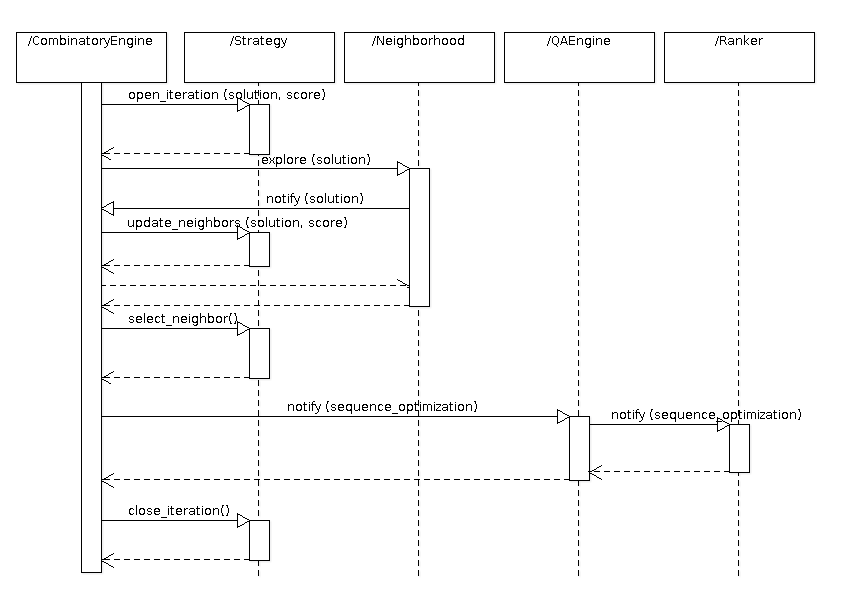
\includegraphics[scale=0.5]{sequence.png}  
  \caption{UML - Pasaje de mensajes}
  \label{uml:sequence}
\end{figure}

\begin{comment}
  \subsection{Interface}
    \paragraph{Responsabilidad:}    
      \begin{enumerate}
       \item 
      \end{enumerate}
    \paragraph{Colaboradores:}
      \begin{enumerate}
       \item 
      \end{enumerate}
\end{comment}
